\section{Zielsetzung}
\label{sec:Zielsetzung}
Es sollen die Kernspins und Land\'e-Faktoren der Rubidium Isotope $^{85}\symup{Rb}$ und $^{87}\symup{Rb}$
durch Ausmessen der Zeemann-Aufspaltung durch ein äußeres Magnetfeld bestimmt werden.

\section{Theorie}
\label{sec:Theorie}
In \autoref{fig:D1} ist eine schematische Darstellung der Elektronenkonfiguration von Rubidum zu sehen.
Diese soll in den folgenden Abschnitten erklärt werden, um das Optische Pumpen theoretisch herzuleiten.

\begin{figure}
    \centering
    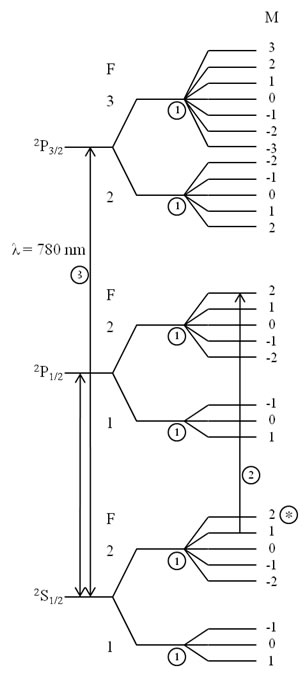
\includegraphics[scale=0.5]{zeeman_splitting.jpg}
    \caption{Schematische Darstellung der Elektronenkonfiguration von Rubidium.\cite{D1}}
    \label{fig:D1}
\end{figure}

\subsection{Quantenzahlen des Atoms}
\label{sec:Quantenzahlen}
Die Energieniveaus eines Atoms lassen sich durch die Hauptquantenzahl $n$, der Bahndrehimpulsquantenzahl $l$
mit $0 \leq l < n$ und der magnetischen Quantenzahl $m$ mit $-l \leq m \leq l$ beschreiben. Rubidium ist ein
Alkalimetall und hat nur ein Valenzelektron, so dass es sich gut durch ein Atom mit einem Elektron annähern lässt.

\subsection{Spin-Bahn-Kopplung}
\label{sec:Spin-Bahn-Kopplung}
Da der Kern im Ruhesystem des Elektrons ein Magnetfeld erzeugt und das Elektron einen Spin hat, spalten sich die
Energieniveaus weiter auf. Dies wird auch Feinstruktur genannt. Die Aufspaltung folgt dem Gesamtdrehimpuls $J$
der sich aus dem Spin und dem Bahndrehimpuls durch $J=L+S$ zusammensetzt. Der Bahndrehimpuls geht von $|L-S|$ bis
$|L+S|$ definiert. Dadurch dass nur ein Valenzelektron vorhanden ist ergibt sich für beide Isotope
$J=S=\frac{1}{2}$.

\subsection{Hyperfeinstruktur}
\label{sec:Hyperfeinstruktur}
Weiterhin gibt es noch eine wesentlich geringere Aufspaltung durch die magnetischen Momente der Kerne. Die
Aufspaltung lässt sich durch die Quantenzahl $F$ beschreiben, die von $|J-I|$ bis $|J+I|$ läuft. Dabei ist
$I$ der Kernspin. Das Isotop $^{85}\symup{Rb}$ hat einen Kernspin von $I=\frac{5}{2}$ und das Isotop
$^{87}\symup{Rb}$ einen Kernspin von $I=\frac{3}{2}$. Mögliche Quantenzahlen sind folglich $F=2$ und $F=3$
für $^{85}\symup{Rb}$ oder $F=1$ und $F=2$ für $^{87}\symup{Rb}$.

\subsection{Zeemanneffekt}
\label{sec:Zeemanneffekt}
Eine weiter Aufspaltung lässt sich durch Einschalten eines externen Magnetfels erreichen. Diese weiter Aufspaltung
der Energieniveaus wird durch die Quantenzahl $M_F$ beschrieben, die durch $-F \leq M_F \leq F$ definiert ist.